\subsubsection{Listar}

  \paragraph{}El listado de matrículas por parte de este usuario es especial,
  ya que es posible realizar un listado de matrículas por asignatura durante un
  curso académico; o bien, realizar el listado solamente con las matrículas de
  un determinado alumno durante un curso académico. Esto permite conocer las
  matriculaciones realizadas en una asignatura durante cierto curso académico,
  o la matriculación particular de un alumno durante un curso académico.

  \paragraph{}Para elegir entre los posibles listados, habrá que seleccionar una
  de las opciones de que aparecen en la figura
  \ref{capturaPantallaOpcionesMatricula}.

  \begin{figure}[!ht]
    \begin{center}
      \fbox{
      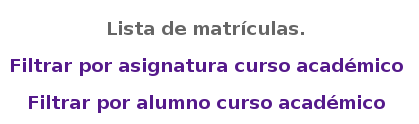
\includegraphics[scale=0.55]{4.Funcionamiento_Aplicacion/4.3.Gestion/4.3.1.Administrador_Principal/4.3.1.13.Matricula/select_listado.png}
      }
      \caption{Captura de pantalla de los enlaces para seleccionar listado de matrícula para el usuario \textit{Administrador principal}.}
      \label{capturaPantallaOpcionesMatricula}
    \end{center}
  \end{figure}

  \paragraph{}Para mostrar la primera lista, es decir, filtrando por asignatura
  curso académico, es necesario establecer el centro para el que mostrar las
  asignaturas curso académico disponibles. Para ello, habrá que elegir el centro
  en la lista desplegable que se muestra en la figura
  \ref{capturaPantallaSelectCentro}.

  \paragraph{}También será necesario elegir la titulación a la que pertenecen
  las asignaturas, por lo que se elegirá entre las opciones de una lista
  desplegable, siguiendo el mismo mecanismo que para seleccionar centro. Se
  puede ver una captura de la selección de titulación en la figura
  \ref{capturaPantallaSelectTitulacion}.

  \paragraph{}Además, habrá que seleccionar la asignatura para la cual se
  listarán los cursos académicos disponibles. Al igual que para la selección de
  centro y de titulación, se seleccionará a través de una lista desplegable con
  las asignaturas disponibles. La figura \ref{capturaPantallaSelectAsignatura}
  muestra una captura de pantalla de esta ventana.

  \paragraph{}Por último, habrá que elegir el curso académico existente para el
  que se realizará el listado de matriculaciones. Se puede ver una captura de
  pantalla de esta ventana en la figura
  \ref{capturaPantallaSelectCursoAcademicoAsignatura}.

  \begin{figure}[!ht]
    \begin{center}
      \fbox{
      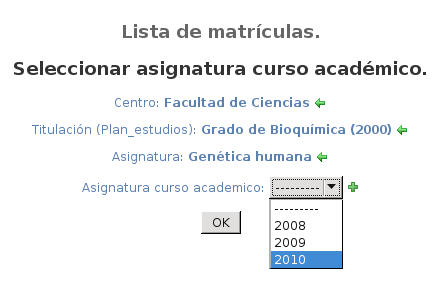
\includegraphics[scale=0.55]{4.Funcionamiento_Aplicacion/4.3.Gestion/4.3.1.Administrador_Principal/4.3.1.13.Matricula/select_cursoAcademico.png}
      }
      \caption{Captura de pantalla de la lista de cursos académico por asignatura para el usuario \textit{Administrador principal}.}
      \label{capturaPantallaSelectCursoAcademicoAsignatura}
    \end{center}
  \end{figure}

  \paragraph{}Nótese que si no existieran elementos disponibles en el sistema,
  la lista desplegable aparecería vacía. Por tanto, se proporciona al usuario
  un icono, representado por una cruz verde, para añadir nuevos elementos al
  sistema. Este icono es el mostrado en la figura \ref{capturaBotonAdd}. Al
  pulsar dicho botón, aparecerá la ventana de creación de un nuevo elemento.

  \paragraph{}Una vez seleccionados el centro, la titulación, la asignatura y
  el curso académico, se muestra la lista completa de matrículas que aparecen en
  el sistema. La figura \ref{capturaPantallaListaMatriculasAdminPrincipal}
  muestra una captura de pantalla de la lista de asignaturas curso académico.

  \begin{figure}[!ht]
    \begin{center}
      \fbox{
      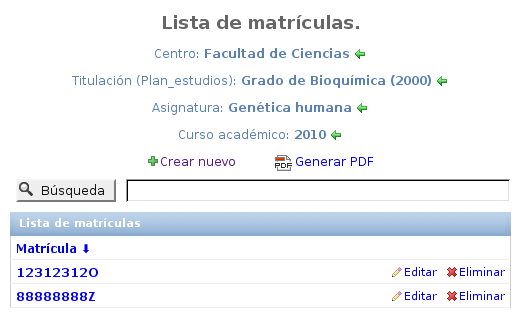
\includegraphics[scale=0.55]{4.Funcionamiento_Aplicacion/4.3.Gestion/4.3.1.Administrador_Principal/4.3.1.13.Matricula/lista_matriculas.png}
      }
      \caption{Captura de pantalla de la lista de matrículas para el usuario \textit{Administrador principal}.}
      \label{capturaPantallaListaMatriculasAdminPrincipal}
    \end{center}
  \end{figure}

  \paragraph{}Si se quisiera refinar el listado de elementos mostrados, es
  posible seleccionar nuevos parámetros pulsando el icono \textit{Seleccionar}
  que aparece al lado de cada elemento. Este icono aparece en la figura
  \ref{capturaBotonSeleccionar}.

  \paragraph{}Para generar el segundo tipo de listado, es decir, por alumno
  durante un determinado curso académico, será necesario seguir el mismo
  procedimiento que acabamos de comentar pero seleccionando el alumno y su curso
  académico, en vez del centro, asignatura y curso académico, como en el primer
  listado.
